\subsection{How much offline knowledge does a static action need, and can the online learner use it?}
\label{sec:granularity}
\paragraph{Question and design} In every battery so far the static competitor was the action validated for each class, the finest offline knowledge a practitioner could have. The comparison with an online learner is fairer, and more useful, when the knowledge is varied: a practitioner may know the size of the instances but not their type, or may meet an instance of a size never tuned for. We ran all $30$ fixed actions of B30 on the $700$ test instances of the standard benchmark (three seeds, $T=1000$; the first $15$ actions are those of B15 and the first five those of B5) and evaluated static policies chosen \emph{only on the tuning instances}, with decreasing knowledge: one action for all instances ($G_0$), one per type ($G_t$), one per size ($G_n$) and one per class ($G_{tn}$, the validated action of Section~\ref{sec:fanjul}). Two transfer regimes drop the tuning data of the tested type ($G_0$ and $G_n$ chosen on the other six types) or of the tested size ($G_0$ and $G_t$ chosen on the other three sizes). A ceiling, the best fixed action per class chosen on two test seeds and evaluated on the third, shows what any class-level static choice can give. The nine predictions $K_1$--$K_9$ and the hashes were recorded before the actions were run on the test instances. (A dry run of the analysis script on $543$ of the $700$ instances, made after that registration to debug the code, showed the pattern of the results; no choice of analysis was changed afterwards.)

\paragraph{Results} Figure~\ref{fig:granularity} and Table~\ref{tab:granularity} give the gains. With no knowledge of the instance at all, one action ($G_0$) gains $1.15$ points in B30, $51\%$ of the class-validated gain ($2.24$), and beats random choice beyond the margin in six of the seven types ($K_1$, $K_2$); the best online learner of each type gains $0.39$ ($17\%$), and none of the seven online learners beats $G_0$ beyond the margin in any of the $49$ learner--type pairs ($K_3$). The size of the instance carries most of the knowledge: $G_n$ recovers $89\%$ of the class-validated gain ($2.00$ points), whereas the type alone adds nothing over $G_0$ ($G_t$: $1.19$) ($K_4$). The class-validated action chosen on $10$ tuning instances per class reaches $99\%$ of the ceiling ($2.24$ against $2.23$; $K_8$). A static action transfers to an unseen \emph{type}: $G_0$ chosen without the type still gains beyond the margin in six of seven types ($1.00$ points) and $G_n$ without the type recovers $87\%$ ($K_5$), and the best online learner beats it in none ($K_6$). It does not transfer to an unseen \emph{size}: $G_0$ and $G_t$ chosen without the tested size gain $0.34$ and $0.38$ points ($15\%$ and $17\%$), and the transferred $G_0$ beats random choice beyond the margin in two of four sizes only ($K_7$ failed). The neural policy of Section~\ref{sec:neural}, which receives $\ln n$ and $\ln m$, gains $1.55$ points ($69\%$) and beats $G_0$ beyond the margin in four of the seven types ($K_9$ failed), consistent with size being the useful knowledge. Seven of the nine predictions held.

\paragraph{Where online learning does pay (post hoc)} The unseen-size regime is the one place where an online learner beats an offline static action. At the two extreme sizes ($n=100$ and $n=1000$, outside the range of the sizes left for tuning) the best online learner beats $G_0$ chosen without that size beyond the margin: at $n=100$ the transferred action \emph{loses} $1.19$ points to random choice while the FRRMAB-style learner is level with it ($+0.07$), and at $n=1000$ the optimistic Q-Learning gains $0.83$ against $0.37$. At the two interior sizes the transferred action wins ($0.84$ and $1.32$ against at most $0.53$). So an online learner is an insurance against a static action that does not cover the instance, never a substitute for one that does: even where it wins, its $0.07$--$0.83$ points are far below the $2.00$ that an action matched to the size gives.

\paragraph{Offline knowledge as the starting point of the online learner (Entries 271 and 272)} The insurance can be built. We warm-started the optimistic Q-Learning with a prior computed on the tuning instances only: the initial value of an action is its score in $[0,1]$ (the best action on the tuning instances scores one, the worst zero) times the optimism factor of the cold learner, the same in all states. With the prior of the instance's type taken from the other sizes (the unseen-size regime) the warm-started learner gains $1.07$ points, against $0.31$ for the cold learner and $0.38$ for the static action chosen without the size; it beats the cold learner beyond the margin in six of the seven types and the transferred static action at all four sizes (at $n=500$ by $0.13$ points, less than the margin). With the prior of the class itself it gains $1.97$ points, $88\%$ of the class-validated gain, and beats the cold learner in all seven types, but never the class-validated action (none of seven). A control with the learning rate set to zero, which keeps the prior and the $5\%$ exploration, shows what learning adds: without it the transferred prior is worth what the transferred static action is worth ($0.40$ against $0.38$) and the class prior what the class-validated action is worth ($2.25$ against $2.24$); learning adds $0.67$ points when the prior was transferred (six of seven types) and costs $0.28$ when the prior was exact. The online learner is therefore best understood as a corrector of offline knowledge: it earns what the prior lacks and pays for what the prior already had. Six of the seven predictions of the warm-start battery held (the miss was a gap of $0.28$ points to the class-validated action against the $0.3$ registered), and all five of the control.

\begin{figure}[t]
\centering
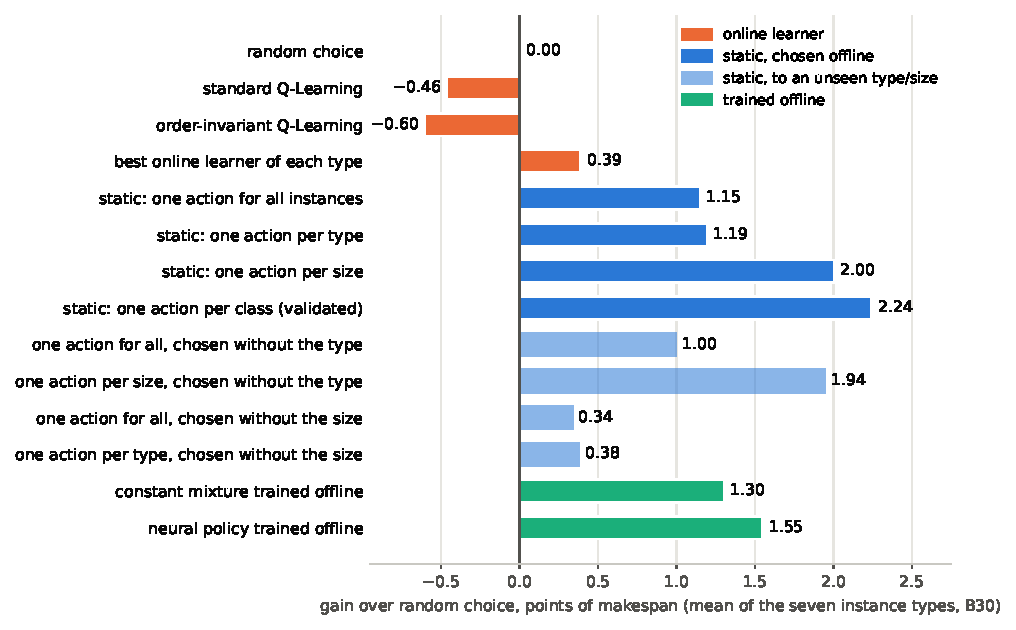
\includegraphics[width=0.92\textwidth]{fig_granularity.pdf}
\caption{The value of offline knowledge by granularity (standard benchmark, B30): gain over random choice, mean of the seven instance types. Orange: online learners; blue: static actions chosen on the tuning instances (hatched: chosen without the type or the size of the instances tested); green: policies trained offline; dotted orange: the optimistic Q-Learning warm-started with an offline prior (and, in blue, the same prior without learning). A single action for all instances beats every online learner; the size of the instance carries most of what class-level knowledge gives.}
\label{fig:granularity}
\end{figure}

% Auto-generated by analysis/make_table_journal.py
\begin{table}[t]
\caption{The value of offline knowledge by granularity on the standard benchmark: gain over random choice (points of makespan; mean of the seven instance types, $100$ test instances each, $T=1000$, three seeds) of static actions chosen on the tuning instances with decreasing knowledge of the instance, of the online learners and of the policies trained offline. B30 also shows the share of the class-validated gain. Static actions are chosen only on the tuning instances; the ceiling chooses on two test seeds and evaluates on the third.}
\label{tab:granularity}
\centering
{\scriptsize\setlength{\tabcolsep}{5pt}
\begin{tabular}{@{}lrrrr@{}}
\toprule
Policy & B5 & B15 & B30 & B30, share of $G_{tn}$ \\
\midrule
random choice & 0 & 0 & 0 & 0 \\
best online learner of each type & 0.22 & 0.31 & 0.39 & 17\% \\
standard Q-Learning & $-$0.33 & 0.05 & $-$0.46 & $-$21\% \\
order-invariant Q-Learning & $-$0.06 & $-$0.24 & $-$0.60 & $-$27\% \\
static, one action for all instances ($G_0$) & 0.28 & 1.02 & 1.15 & 51\% \\
static, by type ($G_t$) & 0.32 & 0.99 & 1.19 & 53\% \\
static, by size ($G_n$) & 0.57 & 1.30 & 2.00 & 89\% \\
static, by class (type, size): the validated action ($G_{tn}$) & 0.87 & 1.60 & 2.24 & 100\% \\
static, by class, chosen on the test seeds (cross-fitted ceiling) & 0.87 & 1.61 & 2.23 & 99\% \\
$G_0$ chosen without the type of the instance & 0.28 & 1.02 & 1.00 & 45\% \\
$G_n$ chosen without the type of the instance & 0.35 & 1.10 & 1.94 & 87\% \\
$G_0$ chosen without the size of the instance & 0.28 & 1.02 & 0.34 & 15\% \\
$G_t$ chosen without the size of the instance & $-$0.40 & 0.33 & 0.38 & 17\% \\
constant mixture trained offline (nn\_const) & -- & 1.03 & 1.30 & 58\% \\
neural policy trained offline (nn) & -- & 1.07 & 1.55 & 69\% \\
\bottomrule
\end{tabular}}
\end{table}



\subsection{What the offline knowledge costs}
\label{sec:cost}
The validated action of a class is chosen with $30$ actions $\times$ $10$ tuning instances $\times$ $2$ seeds, $600$ runs per class, which the comparison at equal iterations does not charge to it. Counted in evaluated moves, estimated from the test runs, they cost $8{,}482$ million moves per class, $11.4$ times the $747$ million of running the validated action once over the $25$ test instances of the class. Resampling the tuning instances (battery 277, existing data only; $1{,}000$ resamples) shows how little of it the knowledge needs (Table~\ref{tab:cost}): with one tuning instance per class ($60$ runs) the class-validated action gains $1.81$ points, $81\%$ of the $2.24$ obtained with ten, and one action per size pooled over the types gains $1.97$ with one instance per class and $2.00$ with ten. Charging the tuning changes the comparison with random choice, whose gap to the best known solutions falls from $7.42\%$ at $10^3$ iterations to $4.31\%$ at $10^4$, against $4.89\%$ for the validated action at $10^3$; random choice at $10^4$ iterations costs $148$ million moves per run. The total cost per instance of the validated action, tuning included, is $29.9+8{,}482/N$ million moves for a class of $N$ instances, which equals the cost of random choice at $10^4$ iterations at $N=72$ and, for the $25$ instances per class of the benchmark, that of random choice at about $25{,}000$ iterations, which a log-linear interpolation of the gap puts near $3.1\%$ (an extrapolation); the interpolated break-even is $130$ instances per class, and $22$ with one tuning instance per class. At $10^4$ iterations the ALNS roulette and the FRRMAB-style learner also end below the validated action at $10^3$ ($3.89\%$ and $4.15\%$). The statement that a validated static action beats every online learner is therefore a statement at a given budget per instance, with the tuning already paid; at a given total compute and a few instances per class, more iterations of random choice are the better use of compute, and the value of offline knowledge lies in amortising it over many instances. Five of the seven predictions registered for this analysis held (the cost ratio, the crossover, the learning curve and its monotonicity, the break-even); the two that missed were that no number of tuning instances would put the static action ahead at the benchmark's own size (one instance per class does, marginally, under the interpolation) and that one action per size would match the class action at three tuning instances ($2.00$ against $2.15$).

\begin{table}[t]
\caption{The price of offline knowledge on the standard benchmark (B30, $T=1000$): the class-validated action chosen with $k$ of the $10$ tuning instances of each class ($1{,}000$ resamples; $k=10$ is the validated action), its gain over random choice (5th--95th percentile of the resamples), its mean gap to the best known solutions, the cost of the tuning in units of one run of the validated action over the $25$ test instances of the class, and the number of instances per class beyond which its total cost, tuning included, is below that of random choice at $T=10^4$ ($4.31\%$ above the best known; measured) and below that of random choice with the iterations that give the same gap (interpolated).}
\label{tab:cost}
\centering
{\scriptsize\setlength{\tabcolsep}{4pt}
\begin{tabular}{@{}rrrrrrr@{}}
\toprule
$k$ & Tuning runs & Gain (p5--p95) & Gap (\%) & Tuning cost & $N$ at $T=10^4$ & $N^*$ \\
\midrule
$1$ & $60$ & $1.81$ ($1.50$--$2.07$) & $5.37$ & $1.2$ & $7$ & $22$ \\
$2$ & $120$ & $2.07$ ($1.79$--$2.20$) & $5.09$ & $2.3$ & $14$ & $32$ \\
$3$ & $180$ & $2.15$ ($2.05$--$2.23$) & $5.00$ & $3.4$ & $22$ & $44$ \\
$5$ & $300$ & $2.21$ ($2.15$--$2.24$) & $4.94$ & $5.7$ & $36$ & $68$ \\
$10$ & $600$ & $2.24$ & $4.90$ & $11.4$ & $72$ & $130$ \\
\bottomrule
\end{tabular}}
\end{table}

